\question Find the path from the start, $S$, to the goal, $G$, when running each of the following algorithms.

\begin{center}
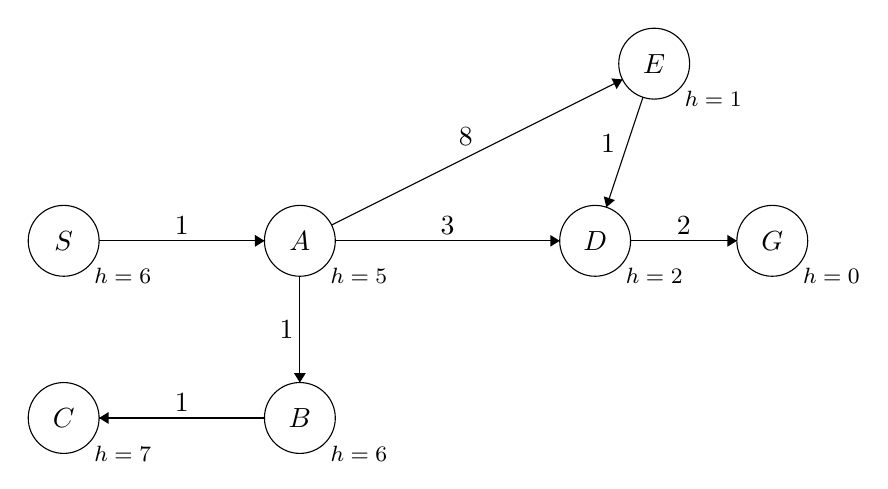
\begin{tikzpicture}[scale=0.15]
\tikzstyle{every node}+=[inner sep=0pt]
\draw (60,-15) circle (3);
\draw (60,-15) node {$E$};
\draw (65,-18) node {\footnotesize $h = 1$};
\draw (10,-30) circle (3);
\draw (10,-30) node {$S$};
\draw (15,-33) node {\footnotesize $h = 6$};
\draw (30,-30) circle (3);
\draw (30,-30) node {$A$};
\draw (35,-33) node {\footnotesize $h = 5$};
\draw (30,-45) circle (3);
\draw (30,-45) node {$B$};
\draw (35,-48) node {\footnotesize $h = 6$};
\draw (55,-30) circle (3);
\draw (55,-30) node {$D$};
\draw (60,-33) node {\footnotesize $h = 2$};
\draw (70,-30) circle (3);
\draw (70,-30) node {$G$};
\draw (75,-33) node {\footnotesize $h = 0$};
\draw (10,-45) circle (3);
\draw (10,-45) node {$C$};
\draw (15,-48) node {\footnotesize $h = 7$};
\draw (13,-30) -- (27,-30);
\fill (27,-30) -- (26.2,-29.5) -- (26.2,-30.5);
\draw (20,-29.5) node [above] {$1$};
\draw (30,-33) -- (30,-42);
\fill (30,-42) -- (30.5,-41.2) -- (29.5,-41.2);
\draw (29.5,-37.5) node [left] {$1$};
\draw (27,-45) -- (13,-45);
\fill (13,-45) -- (13.8,-45.5) -- (13.8,-44.5);
\draw (20,-44.5) node [above] {$1$};
\draw (33,-30) -- (52,-30);
\fill (52,-30) -- (51.2,-29.5) -- (51.2,-30.5);
\draw (42.5,-29.5) node [above] {$3$};
\draw (32.68,-28.66) -- (57.32,-16.34);
\fill (57.32,-16.34) -- (56.38,-16.25) -- (56.82,-17.15);
\draw (44.04,-22) node [above] {$8$};
\draw (59.05,-17.85) -- (55.95,-27.15);
\fill (55.95,-27.15) -- (56.68,-26.55) -- (55.73,-26.24);
\draw (56.73,-21.8) node [left] {$1$};
\draw (58,-30) -- (67,-30);
\fill (67,-30) -- (66.2,-29.5) -- (66.2,-30.5);
\draw (62.5,-29.5) node [above] {$2$};
\end{tikzpicture}
\end{center}

\vspace{\parskip}

\begin{solution}
Note that uniform cost search and greedy search are not a part of the course. The algorithms for all 3 of these searches are extremely similar, the only difference being the priority given to a key and whether or not we need the cumulative distance to a vertex.
\end{solution}

\begin{parts}
\part Which path does uniform cost search return?
\begin{solution}[1.5in]
$S - A - D - G$

From the starting node, choose the path that has the least cost, go to that node, and repeat until we reach the goal node. We choose the lowest \textit{backward cost}.

Note that this is very similar to Dijkstra's, just a little more general. We keep a priority-queue fringe that keeps track of paths. At each step, we remove the shortest path from the fringe and add its children to the fringe, trying all paths in increasing cost order until we reach G.
\end{solution}

\part Which path does greedy search return?
\begin{solution}[1.5in]
$S - A - E - D - G$ or $S - A - D - G$ depending on tie-breaking behavior.

From the starting node, travel to the next node with the lowest value returned by the heuristic function until we reach the goal node. We choose the path with the lowest \textit{forward cost}.
\end{solution}

\part Which path does A* search return?
\begin{solution}[1.5in]
$S - A - D - G$

At each node, we choose the next node that has the lowest sum of the path cost and $h(\cdot)$ value. This is essentially uniform cost search and greedy search combined.

\end{solution}
\end{parts}